\begin{problem}
\textbf{\textsc{Motorized Pendulum 1}}
A pendulum is made of a massless rod of length $l=0.5000\;\mathrm{m}$ and a point mass $m=15.00\;\mathrm{kg}$ hanging at one end. The angle between the rod and the vertical is $\theta$. A motor attached to the pivot supplies a torque. The maximum value of this torque is angle-dependent and is given by $\tau (\theta)=\frac{1+\cos\theta}{2} \tau_0$ for $0\leq \theta \leq 90^{\circ}$.

\begin{figure}[h]
    \centering
    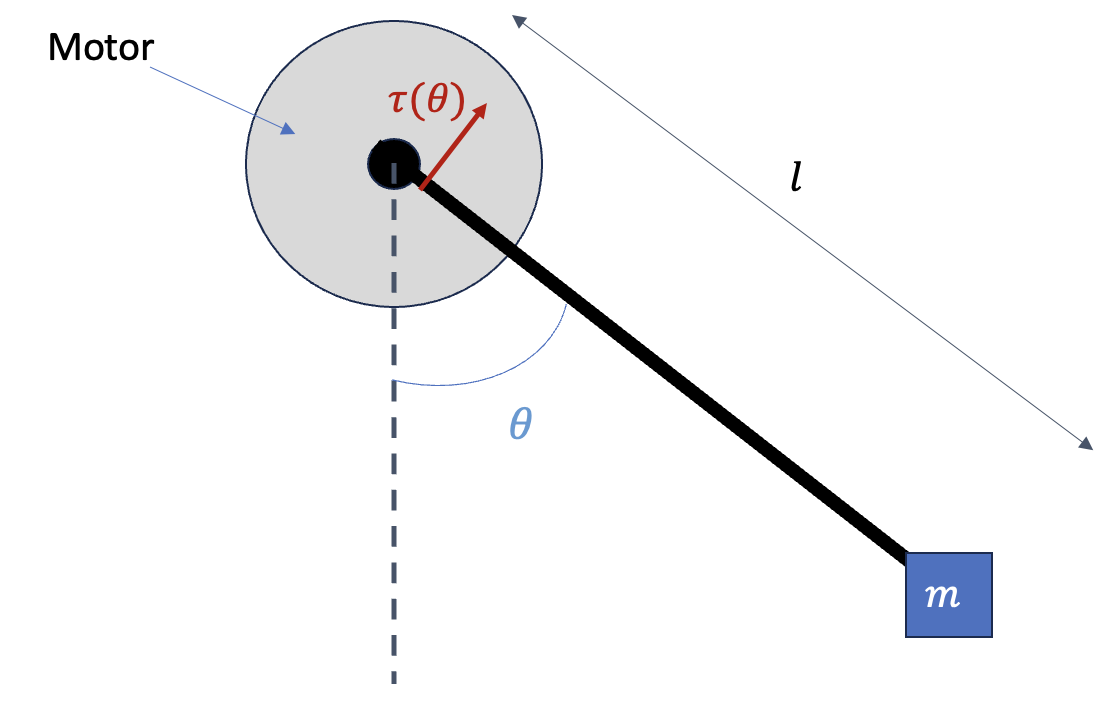
\includegraphics[width=0.5\linewidth]{problems/figures/mot_pend.png}
    \caption{Motorized pendulum}
    \label{fig:enter-label}
\end{figure}

The pendulum initially is given a small angular velocity counterclockwise and is at $\theta = 0$. The mass is extremely sensitive and cannot tolerate high speeds. Therefore, assume the motor always supplies just enough torque for the mass to move at a negligibly small constant speed. What is the minimum value of $\tau_0$ needed so that the pendulum eventually reaches $\theta=90^{\circ}$?


\end{problem}